\chapter{Results}
\begin{figure}[ht]
\centering
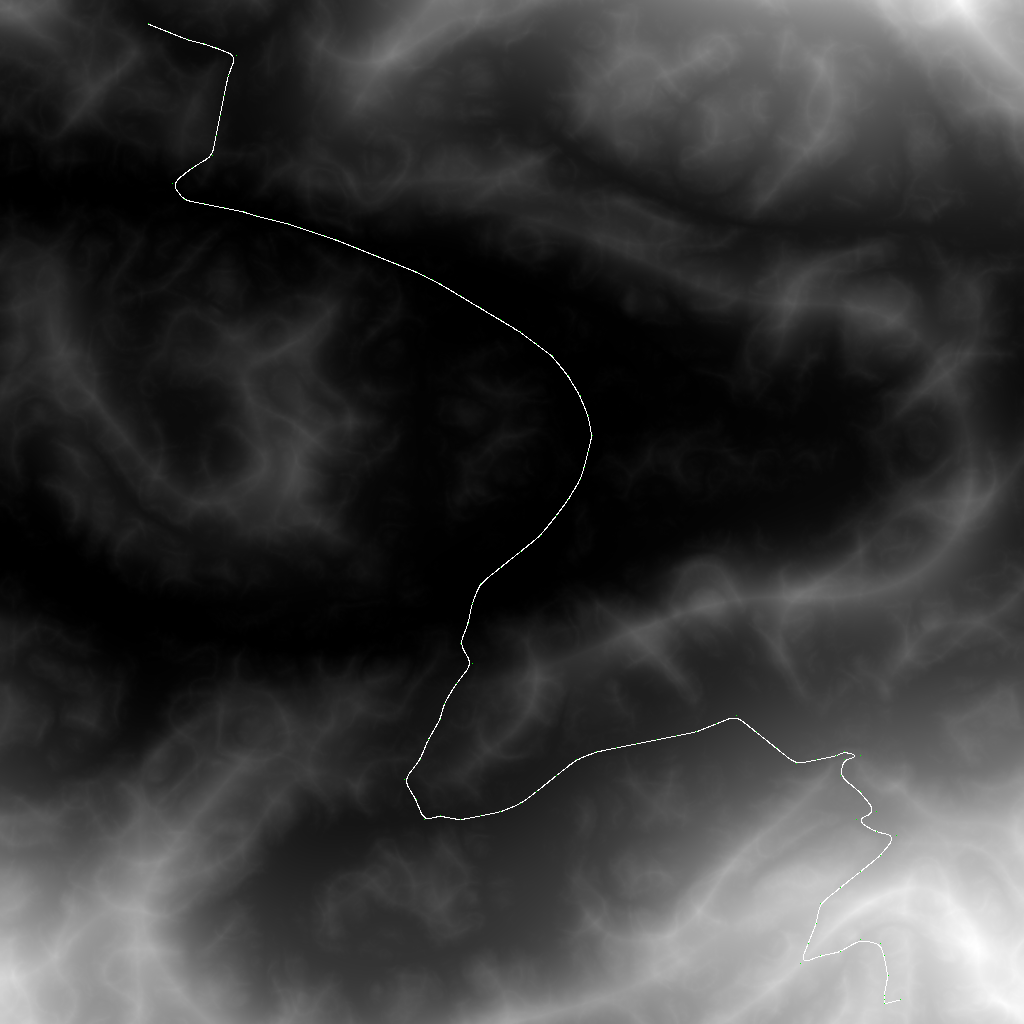
\includegraphics[width=0.5\textwidth]{figure/generated_road_trajectory}
\caption{A procedurally generated road trajectory}
\label{fig:road_trajectory}
\end{figure}

\section{Performance of road generator}

\section{Visual results}
After loading the model into the snow simulator and adjusting the terrain, we can see the roads as it curves through the terrain. Figure \ref{fig:road_in_terrain_nosnow} shows the road and the terrain without snow cover. We clearly see the effects of the terrain adjustments in the bottom two screenshots, i.e. figures \ref{fig:road_in_terrain_nosnow_2} and \ref{fig:road_in_terrain_nosnow_3}. Note that snow rendering was disabled on the overview image (figure \ref{fig:road_in_terrain_nosnow_1}) in order to improve visibility of the road.

\begin{figure}[ht]
\centering
\subfloat[Terrain overview]{\label{fig:road_in_terrain_nosnow_1}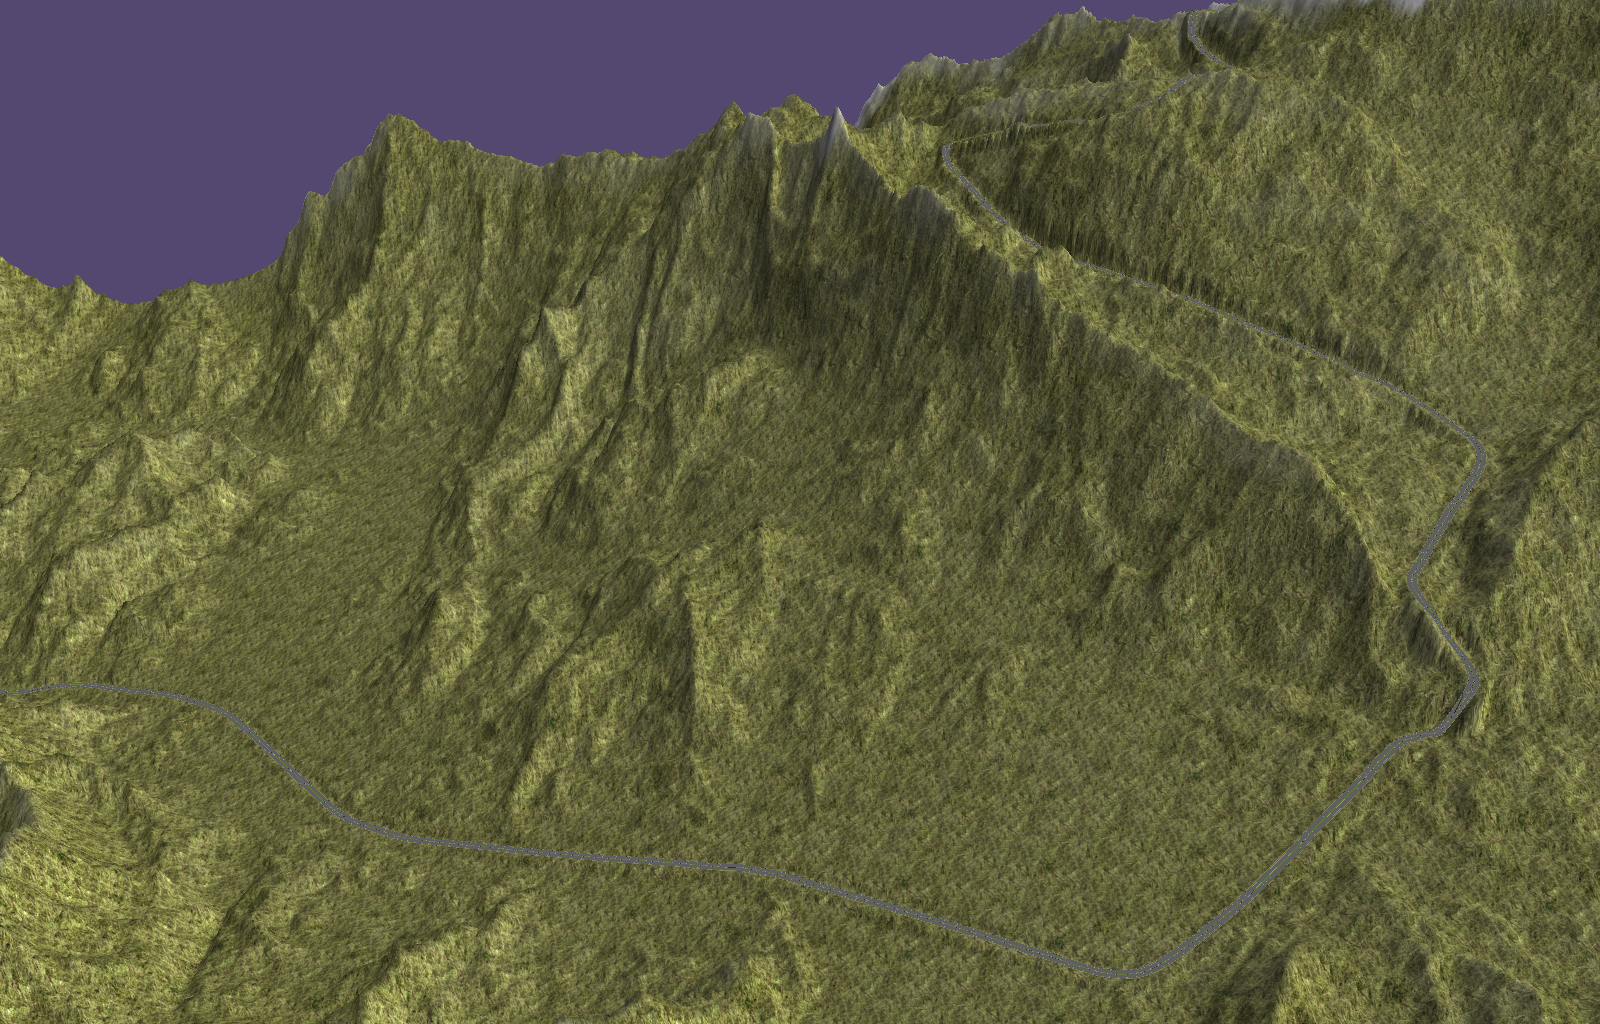
\includegraphics[width=\textwidth]{figure/screenshots/road_nosnow_1}}\\
\subfloat[Detailed view of road]{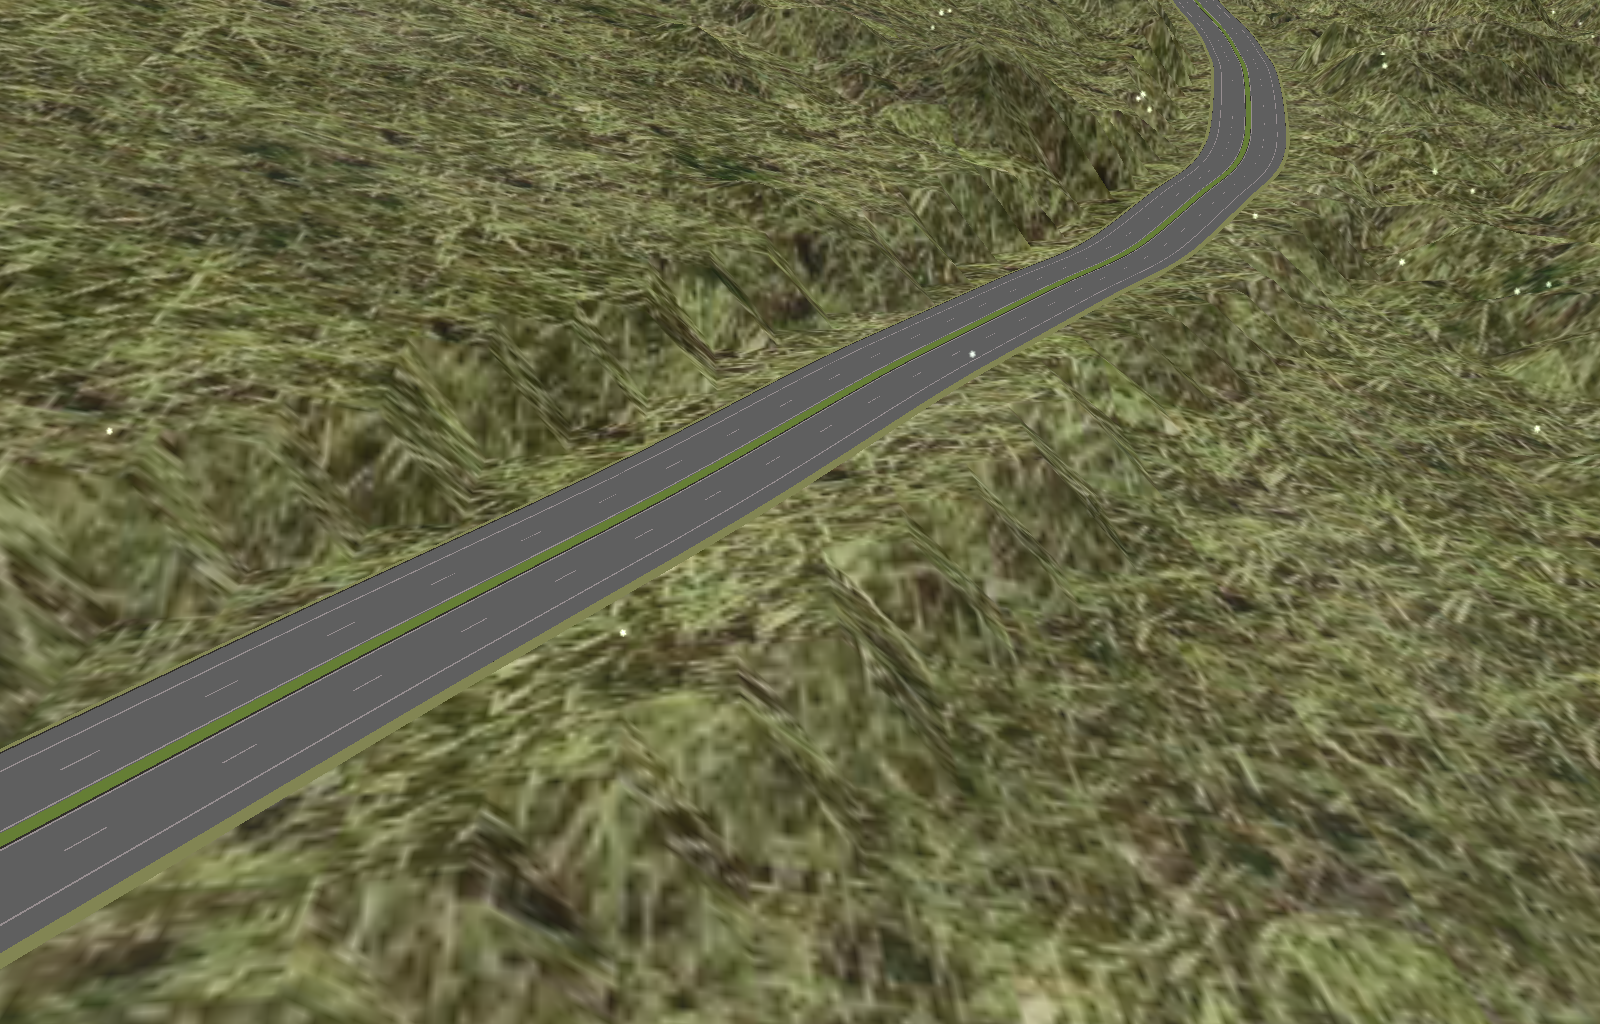
\includegraphics[width=0.485\textwidth]{figure/screenshots/road_nosnow_2}}\quad
\subfloat[Significant terrain adjustments]{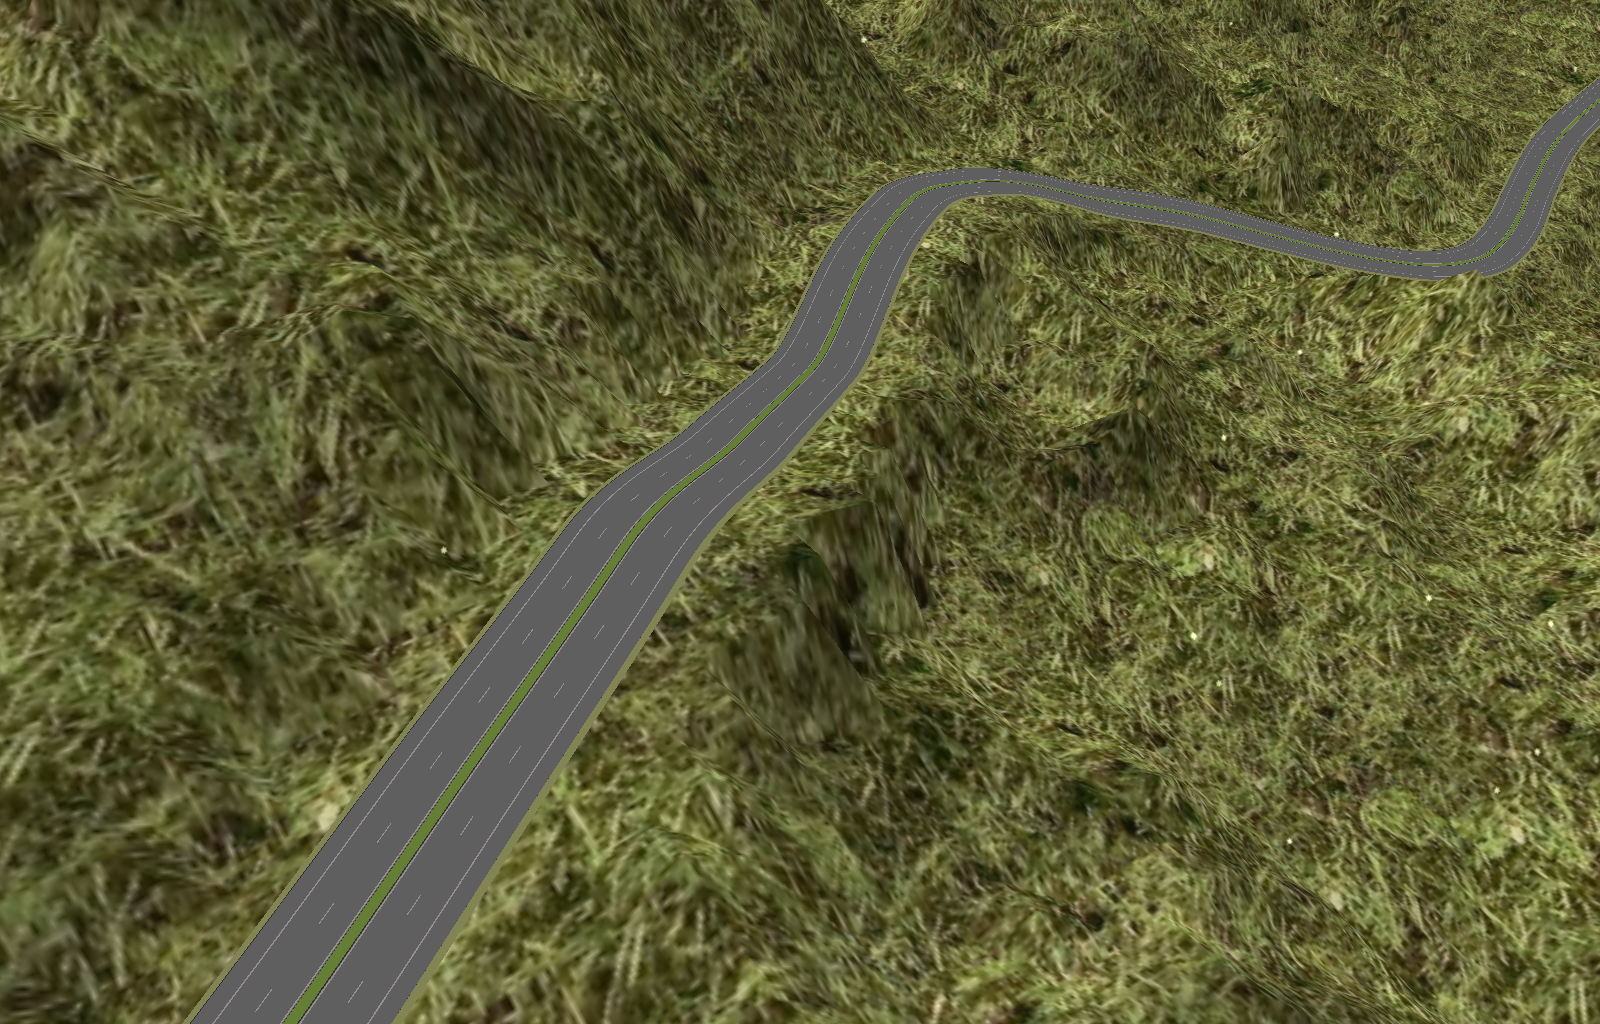
\includegraphics[width=0.485\textwidth]{figure/screenshots/road_nosnow_3}}
\caption{Road and terrain before snowcover}
\label{fig:road_in_terrain_nosnow}
\end{figure}

After some snow has fallen, as in figure \ref{fig:road_in_terrain_nosnow}, the terrain has been more or less covered in snow except for some shadowed areas. The snow height is continously "smoothed", so that snow that falls in areas with a steep gradient in the terrain, is moved downwards along the gradient, simulating sliding snow (think of it as a mini avalanche). We clearly see this effect on the road in figures \ref{fig:road_in_terrain_nosnow_2} and \ref{fig:road_in_terrain_nosnow_3}.

\begin{figure}[ht]
\centering
\subfloat[Snow covered terrain overview]{\label{fig:road_in_terrain_nosnow_1}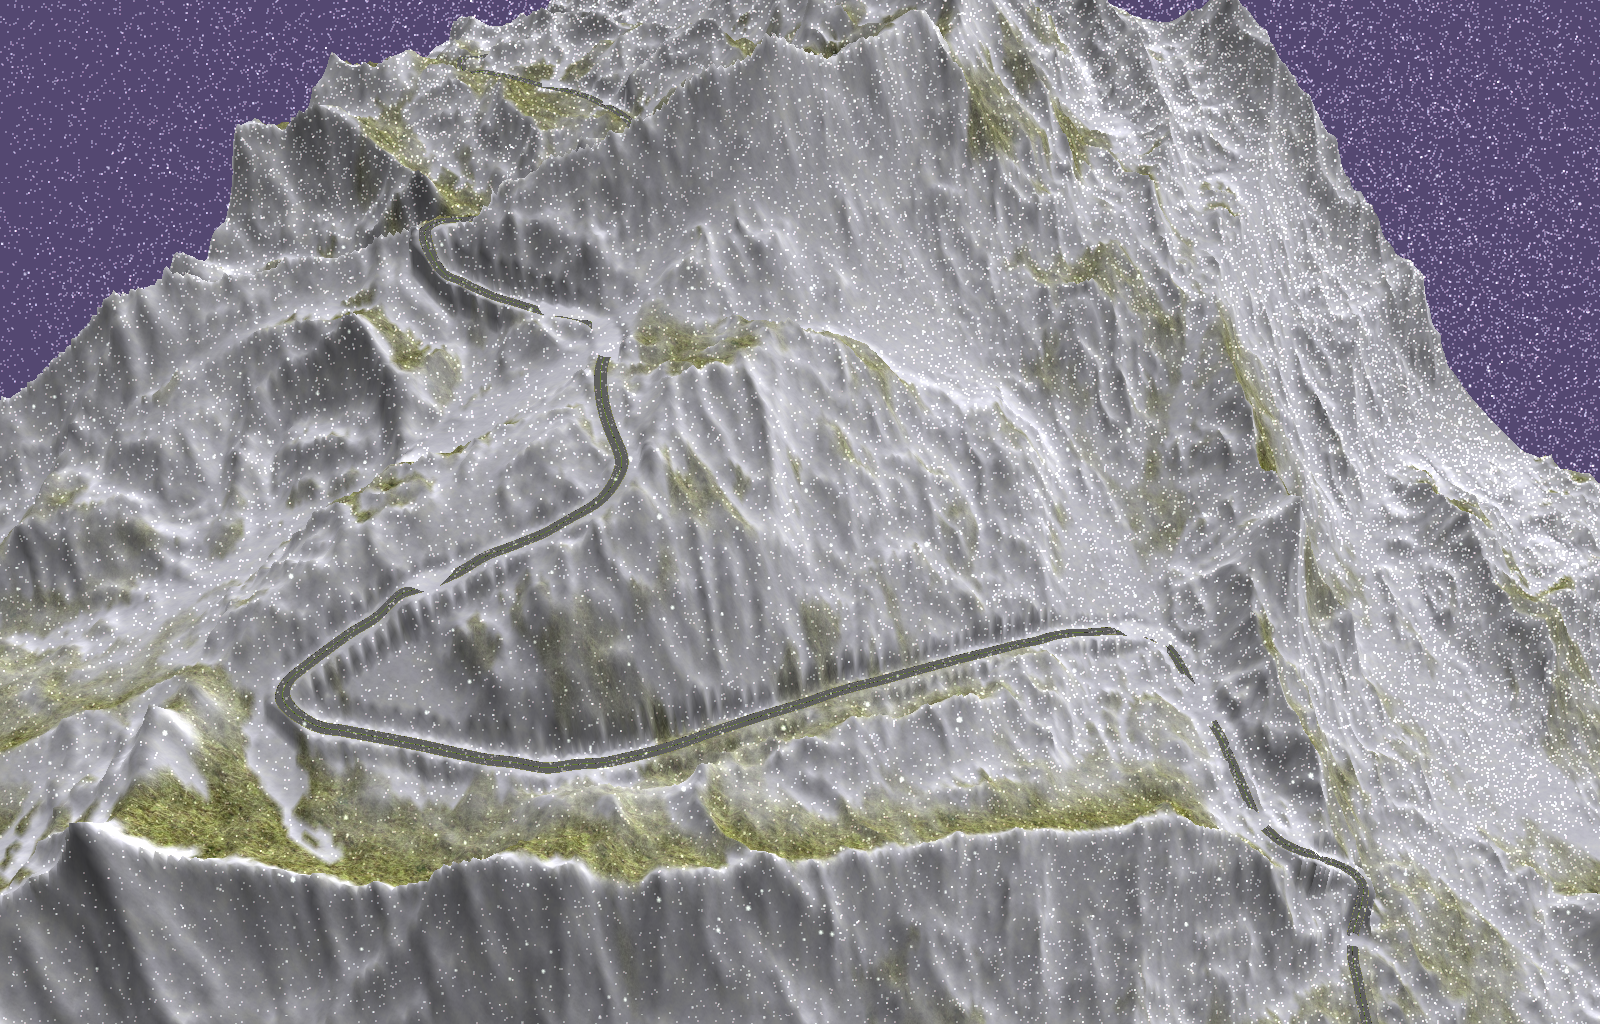
\includegraphics[width=\textwidth]{figure/screenshots/road_snow_1}}\\
\subfloat[Snow from higher up covering road]{\label{fig:road_in_terrain_nosnow_2}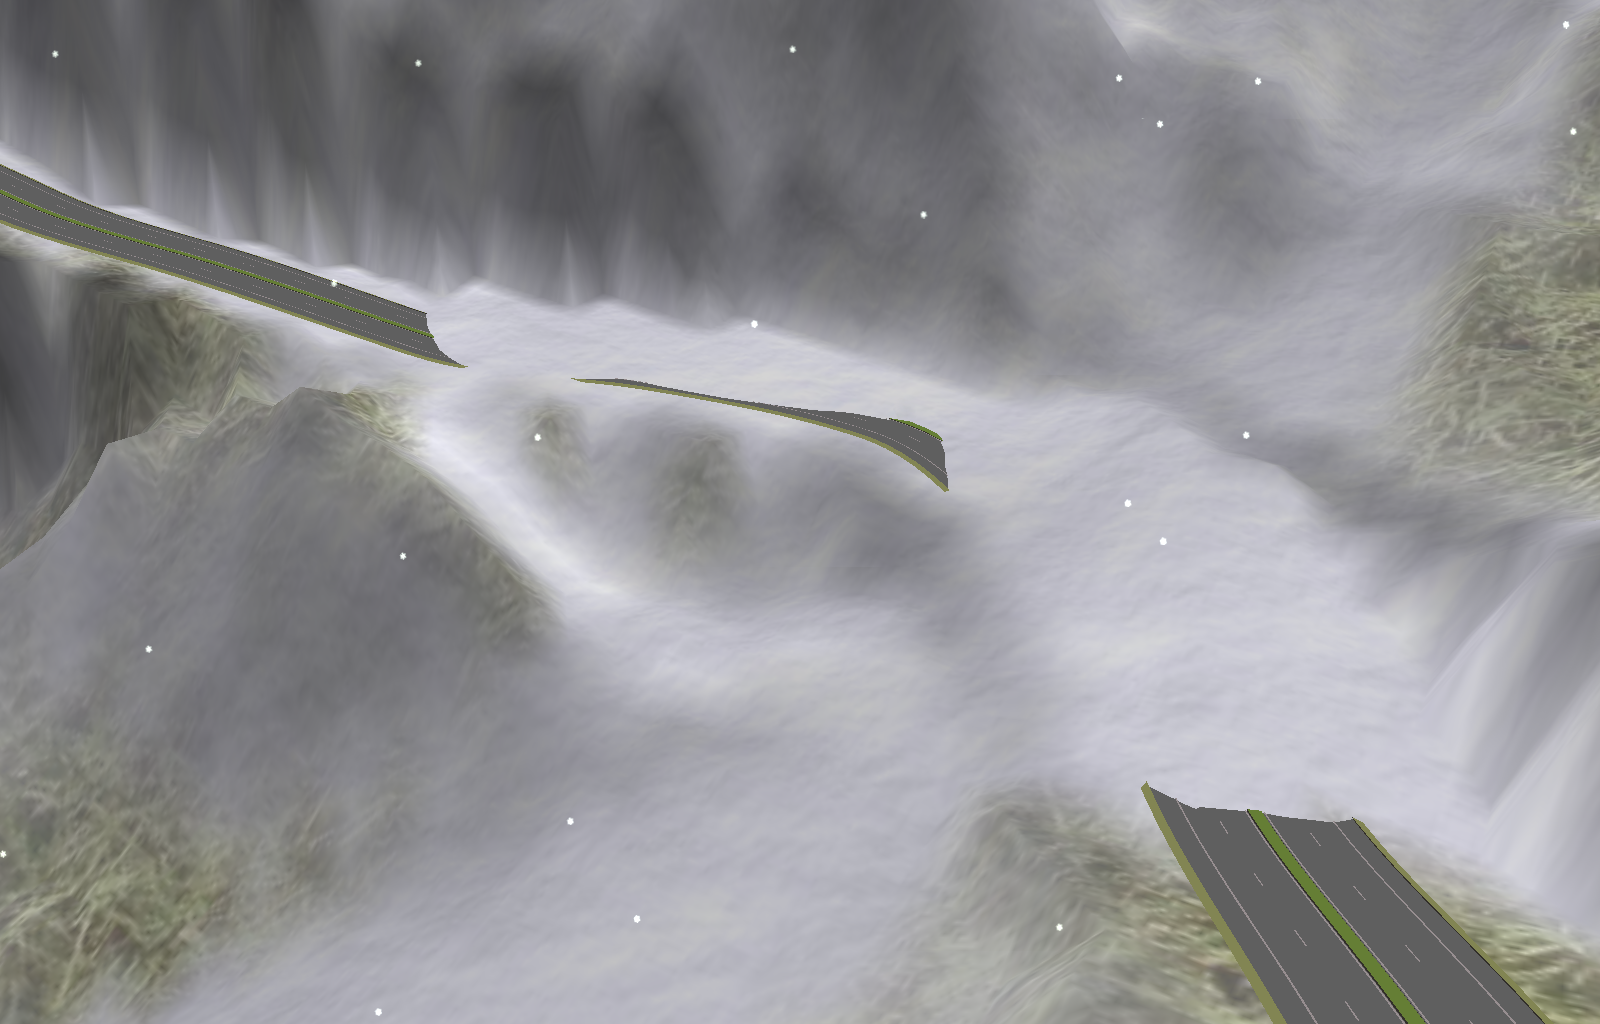
\includegraphics[width=0.485\textwidth]{figure/screenshots/road_snow_2}}\quad
\subfloat[Another case of snow sliding down on the road]{\label{fig:road_in_terrain_nosnow_3}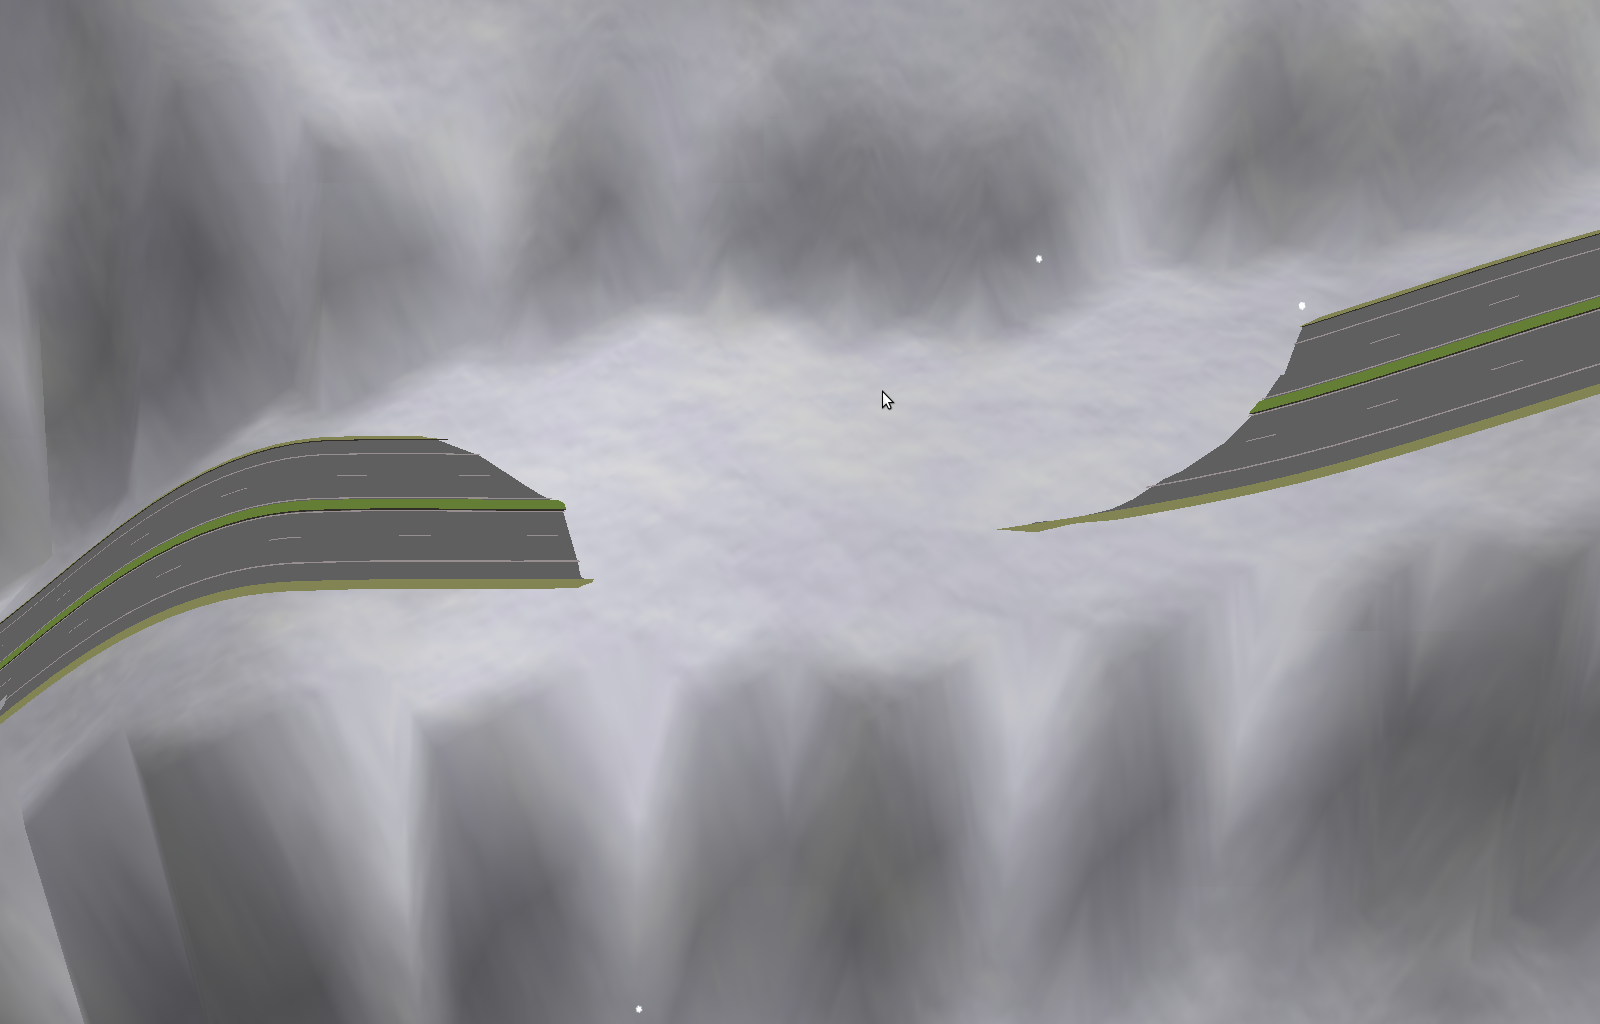
\includegraphics[width=0.485\textwidth]{figure/screenshots/road_snow_3}}
\caption{Road and terrain with snowcover}
\label{fig:road_in_terrain_snow}
\end{figure}
